%!TEX root = ../thesis.tex
\chapter{Fundamentals}
\label{ch:fundamentals}

\section{Computer Vision}
\label{sec:computer-vision}

\textcite{Goodfellow-et-al-2016} describe vision as a capability that is effortless and automatic for humans and animals, yet one that has historically proven difficult to formalize in computational systems. \textcite{hartley_multiple_2003} frame the core goal of the field simply as "making a computer see." Szeliski gives this a more concrete shape, characterizing computer vision as an inverse problem: given one or more images, the task is to recover the physical properties that produced them — shape, illumination, color — from information that is inherently insufficient to determine a unique solution \parencite{szeliski_computer_2022}. Because no single answer follows directly from the image data alone, this ambiguity must be resolved by falling back on physics-based models, probabilistic frameworks, or machine learning trained on large exemplar datasets. This inverse-problem view is also what conceptually separates computer vision from digital image processing: rather than only transforming pixel values, computer vision aims to recover the three-dimensional structure of a scene as a step toward high-level scene understanding \parencite{szeliski_computer_2022}.

\section{Object Detection}
\label{object-detection}

\textcite{zou_obj_2023} define object detection as the task of finding instances of specific object classes, such as humans, animals, or vehicles, in an image. They reduce this task to a single question: "What objects are where?" 
\textcite{szeliski_computer_2022} gives a more concrete definition: object detection means drawing a bounding box around each recognized object in an image. \textcite{Goodfellow-et-al-2016} view object recognition and detection as central to deep learning in CV, and argue that progress on these tasks has driven much of the field's architectural development. Object detection models are typically evaluated on two measures: accuracy and speed \parencite{zou_obj_2023}. Accuracy covers both classification (what is it?) and localization (where is it?). The task also underlies other applications, such as instance segmentation, image captioning, and object tracking, and involves recurring challenges, including objects at different scales, rotation, heavy occlusion, and real-time execution speed \parencite{zou_obj_2023}.

Before 2014, object detection relied on handcrafted features and carefully engineered rules, since no method yet existed to learn a useful representation directly from data \parencite{zou_obj_2023}. \textcite{zou_obj_2023} trace this traditional period through three milestones. The Viola-Jones detector (2001) used a sliding window and a cascade of simple classifiers to achieve real-time face detection. The Histogram of Oriented Gradients (HOG) detector (2005) computed dense gradient features across an image and became a standard baseline for pedestrian detection. The Deformable Part-based Model (DPM), developed between 2008 and 2010, represented objects as a collection of deformable parts and is considered the high point of the traditional era.

\textcite{Goodfellow-et-al-2016} explain why this reliance on handcrafted features was limiting: designing a feature by hand, such as a rule for recognizing a wheel, is labor-intensive and does not transfer well to other tasks or object classes. Even a feature as simple as a wheel is hard to define directly in pixel values once shadows, glare, and occlusion are taken into account. Deep learning replaced this hand engineering with automatic feature learning, building up simple edges into contours, contours into object parts, and object parts into full object identities. This shift became visible in 2012, when a deep convolutional network won the ImageNet Large Scale Visual Recognition Challenge by a wide margin, cutting the top-5 error rate from 26.1 \% to 15.3 \% \parencite{Goodfellow-et-al-2016}.

\begin{figure}[ht]
    \centering
    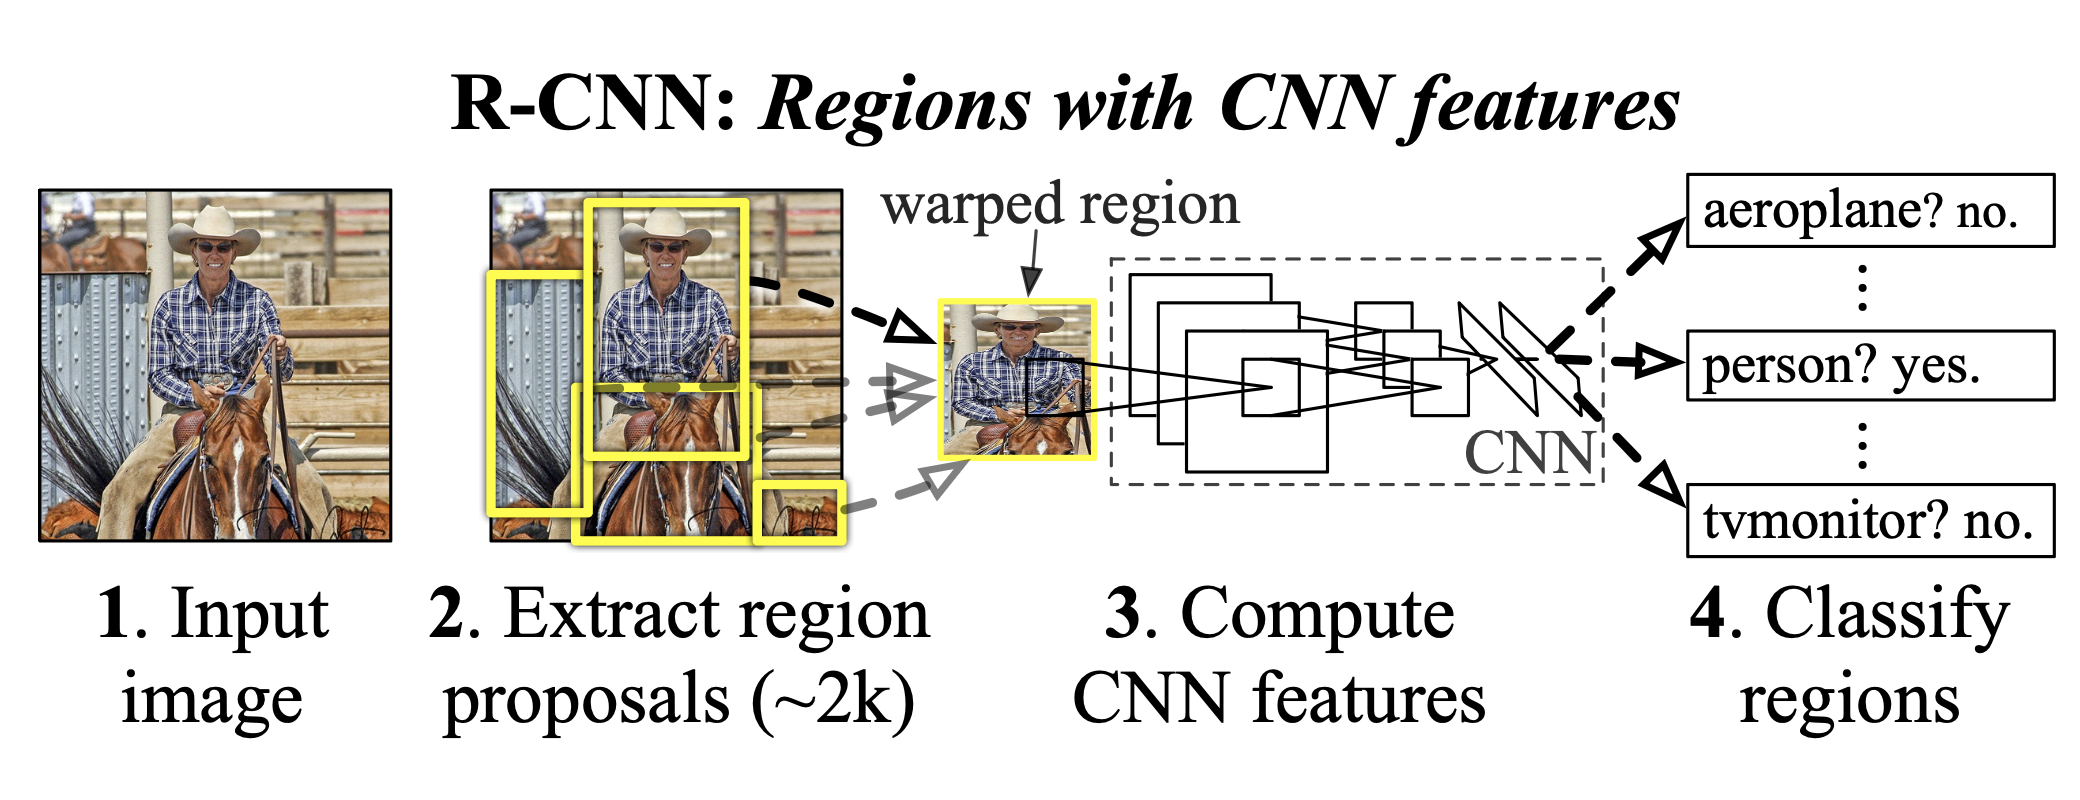
\includegraphics[width=\textwidth, height=\textheight, keepaspectratio]{figures/gershick_R-CNN.png}
    \caption{Object detection system overview \textcite{girshick_2014_rcnn}}
    \label{fig:rcnn}
\end{figure}

This success carried directly into object detection. \textcite{zou_obj_2023} identify Girshick et al.'s R-CNN (\ref{fig:rcnn}) \parencite{girshick_2014_rcnn} as the watershed detector that triggered the transition to deep learning. Operating within the "recognition using regions" paradigm, R-CNN bypassed the computational limits of sliding-window CNNs by extracting approximately 2,000 category-independent bottom-up region proposals per image via Selective Search. Each proposal was context-dilated ($p=16$ pixels), warped to a uniform $227 \times 227$ resolution, and forward-propagated through a 5-layer convolutional network to yield a 4,096-dimensional feature vector. These vectors were classified using class-specific linear Support Vector Machines (SVMs) and refined via post-hoc bounding box regression. Crucially, Girshick et al. demonstrated that supervised pre-training on ImageNet followed by domain-specific fine-tuning on detection targets yielded an 8 percentage point boost in accuracy, raising PASCAL VOC07 performance from 33.7\% (DPM) to 58.5\% mAP. However, forward-propagating 2,000 isolated regions per image introduced substantial computational redundancy, creating a severe speed bottleneck ($\sim$13s/image on GPU) that spurred subsequent feature-sharing architectures \parencite{girshick_2014_rcnn}. This propose-then-classify approach, later refined into SPPNet, Fast R-CNN, and Faster R-CNN, became known as two-stage detection. A second family of detectors instead skipped the proposal step, predicting boxes and classes directly in a single pass to trade some accuracy for speed \parencite{zou_obj_2023}. \textcite{redmon_you_2016}, by the introduction of You Only Look Once (YOLO), fundamentally departed from this multi-stage pipeline by framing object detection as a single regression problem, mapping directly from raw image pixels to bounding box coordinates and class probabilities within a single evaluation pass  was the first detector to popularize this one-stage approach \parencite{redmon_you_2016}.

\section{Convolutional Neural Networks}
\label{sec:cnn}

Convolutional Neural Networks (CNNs) represent a specialized class of artificial neural networks designed specifically for processing data structured in a grid-like topology, such as two-dimensional spatial pixel arrays in digital imagery \parencite{Goodfellow-et-al-2016}. Fundamentally, a CNN is defined as any neural network architecture that employs the mathematical linear operation of convolution in place of general matrix multiplication in at least one of its constituent layers \parencite{Goodfellow-et-al-2016}.

The foundational architecture of CNNs is directly motivated by neuroscientific discoveries regarding the mammalian visual cortex, specifically the physiological findings of Hubel and Wiesel \parencite{hubel_receptive_1962, Goodfellow-et-al-2016}. In their foundational recordings of individual cortical neurons, Hubel and Wiesel observed that visual processing relies on spatially localized receptive fields that activate in response to highly specific stimuli, such as oriented light bars or edges \parencite{hubel_receptive_1962, Goodfellow-et-al-2016}. Crucially, they categorized these visual neurons into two main functional types in the primary visual cortex (V1): simple cells, which perform localized, linear feature extraction over small receptive fields, and complex cells, which pool responses from multiple simple cells across local spatial neighborhoods to achieve shift invariance and robustness to minor spatial displacements \parencite{Goodfellow-et-al-2016, scherer_evaluation_2010}. This biological functional split established the core architectural paradigm of alternating local feature detection and spatial aggregation that governs modern convolutional processing \parencite{Goodfellow-et-al-2016, scherer_evaluation_2010, lecun_gradient-based_1998}.

This biological model was first translated into a computational framework by Fukushima through the Neocognitron, which serves as the direct structural precursor to modern CNN architectures \parencite{fukushima_neocognitron_1980, scherer_evaluation_2010, lecun_gradient-based_1998}. The Neocognitron instantiated Hubel and Wiesel's physiological concepts via a cascaded, multi-stage network composed of modular layers: S-layers containing S-cells (emulating simple cells for localized feature extraction) alternated with C-layers containing C-cells (emulating complex cells for position-tolerant aggregation) \parencite{fukushima_neocognitron_1980}. The architecture explicitly introduced localized receptive fields, weight sharing across units in a cell-plane to detect identical features at varying spatial coordinates, and progressive spatial downsampling \parencite{fukushima_neocognitron_1980}. Although the Neocognitron relied on layer-wise unsupervised learning rather than global supervised backpropagation, its structural hierarchy directly defined the alternating convolution and pooling mechanics utilized in contemporary deep visual architectures \parencite{fukushima_neocognitron_1980, Goodfellow-et-al-2016, lecun_gradient-based_1998}.

\subsection{The Convolution Operation}

The convolution operation forms the computational backbone of modern visual architectures, replacing general matrix multiplication with localized kernel operations \parencite{Goodfellow-et-al-2016}. In visual processing, inputs are structured as multi-channel three-dimensional tensors, where spatial coordinates $(j,k)$ are augmented by a channel axis $l$ representing input color channels or feature maps from preceding layers \parencite{Goodfellow-et-al-2016}. A convolutional layer applies a four-dimensional parameter tensor---termed the kernel or filter---where kernel coefficients $K_{i,l,m,n}$ define the learned connection weights from input channel $l$ at spatial offset $(m,n)$ to output feature map channel $i$ \parencite{Goodfellow-et-al-2016}. Formally, for an input tensor $V$, kernel tensor $K$, and spatial stride $s$, the discrete strided multi-channel convolution operation producing output feature map tensor $Z$ at location $(i,j,k)$ is expressed as \parencite{Goodfellow-et-al-2016}:

\begin{equation}
Z_{i,j,k} = \sum_{l} \sum_{m} \sum_{n} V_{l,\,(j-1)s+m,\,(k-1)s+n} \, K_{i,l,m,n}
\label{eq:conv}
\end{equation}

The spatial stride parameter $s$ governs the discretization step size as the kernel slides across the spatial grid, where $s > 1$ performs explicit spatial downsampling during feature extraction \parencite{Goodfellow-et-al-2016}. To handle boundaries, zero-padding appends implicit zeros surrounding the spatial borders of the input tensor $V$, allowing direct control over output spatial dimensions \parencite{Goodfellow-et-al-2016}. Without padding (valid convolution), spatial dimensions shrink by $k-1$ at every layer for a kernel of spatial width $k$, strictly limiting total network depth before the spatial map collapses to $1 \times 1$ \parencite{Goodfellow-et-al-2016}. By contrast, applying sufficient zero-padding (same convolution) keeps input and output spatial dimensions identical, enabling the construction of arbitrarily deep convolutional hierarchies \parencite{Goodfellow-et-al-2016}.

Beyond reducing memory consumption and arithmetic complexity, the convolution operation enforces three fundamental structural properties---acting as an infinitely strong prior---that make it uniquely adapted to processing spatial image data \parencite{Goodfellow-et-al-2016}:

\begin{itemize}
    \item \textbf{Sparse Connectivity (Local Interactions):} Unlike traditional fully connected layers that compute global matrix-vector products across all inputs, convolutional layers enforce sparse interactions \parencite{Goodfellow-et-al-2016}. Each unit in an output feature map receives inputs only from a small, spatially contiguous local patch of the preceding layer, known as its local receptive field \parencite{Goodfellow-et-al-2016, lecun_backpropagation_1989, lecun_gradient-based_1998}. This mirrors the spatial structure of natural images, where spatially proximate pixels exhibit strong statistical dependencies while distant pixels are largely uncorrelated \parencite{Goodfellow-et-al-2016, lecun_gradient-based_1998}.

    \item \textbf{Parameter Sharing:} Convolution incorporates weight sharing, enforcing the constraint that all spatial units within a given feature map share an identical set of kernel weights $K_{i,l,m,n}$ \parencite{Goodfellow-et-al-2016, lecun_backpropagation_1989, lecun_gradient-based_1998}. This reflects the spatial prior that local visual features (e.g., edges, contours, or textures) are statistically stationary across the visual field, meaning a feature detector optimized to detect a specific pattern at one spatial coordinate is functional across all spatial coordinates \parencite{Goodfellow-et-al-2016, lecun_backpropagation_1989}.

    \item \textbf{Translation Equivariance:} Parameter sharing across a regular grid guarantees mathematical equivariance to translation, defined such that a transformation $g$ applied to input image $x$ commutes with the feature mapping function $f$, satisfying $f(g(x)) = g(f(x))$ \parencite{Goodfellow-et-al-2016}. Specifically, if an input visual stimulus is shifted spatially by a translation vector, the resulting output feature map shifts by the exact same vector without altering the internal feature activation values \parencite{Goodfellow-et-al-2016}.
\end{itemize}

Together, these three inductive biases embed spatial locality and translation invariance directly into the neural network's structural graph, rendering convolutional architectures exponentially more parameter-efficient and statistically powerful for visual pattern recognition than unstructured fully connected networks \parencite{Goodfellow-et-al-2016, lecun_backpropagation_1989, lecun_gradient-based_1998}.

\subsection{Pooling and Downsampling}

Following feature extraction in the convolutional detector stage, pooling operations are applied to aggregate spatial activations across localized neighborhoods, replacing exact pixel-level feature locations with summary statistics \parencite{Goodfellow-et-al-2016, scherer_evaluation_2010}. The two primary mathematical formulations of spatial pooling are max pooling and average pooling \parencite{Goodfellow-et-al-2016, scherer_evaluation_2010, Boureau_CNN_2010}. Max pooling calculates the maximum activation value within a local rectangular window, isolating the most dominant feature response while suppressing background noise \parencite{Goodfellow-et-al-2016, scherer_evaluation_2010, Boureau_CNN_2010}. Average pooling (historically implemented in early architectures such as LeNet-5 as trainable subsampling) computes the spatial arithmetic mean over the pooling window, yielding a smoothed, low-pass representation of local feature responses \parencite{Goodfellow-et-al-2016, scherer_evaluation_2010, lecun_gradient-based_1998}.

While early convolutional frameworks relied heavily on trainable average subsampling \parencite{lecun_gradient-based_1998}, subsequent theoretical and empirical analyses demonstrate that max pooling is vastly superior for capturing spatial invariances and preserving discriminative feature signatures, particularly when operating on sparse feature codes \parencite{scherer_evaluation_2010, Boureau_CNN_2010}. A slight contradiction arises between early architectural paradigms and modern empirical findings: early designs treated pooling as a trainable, linear averaging filter with sigmoidal squashing \parencite{lecun_gradient-based_1998}, whereas comparative evaluations show that parameter-free, non-linear max pooling provides stronger invariance and superior classification accuracy without requiring additional learned parameters \parencite{scherer_evaluation_2010, Boureau_CNN_2010}. Furthermore, pooling windows can be arranged as non-overlapping contiguous regions or as overlapping pooling regions where the spatial stride is smaller than the pooling window size ($s < z$), a configuration that enhances feature generalization and makes models less prone to overfitting \parencite{Krizhevsky_ImageNET}.

The integration of pooling layers into deep convolutional architectures is justified by three distinct functional and structural benefits:

\begin{itemize}
    \item \textbf{Local Translation Invariance:} While convolutional layers achieve translation equivariance (shifting an input image shifts its corresponding output feature map identically) \parencite{Goodfellow-et-al-2016, nair_relu_2010}, pooling layers convert this behavior into local translation invariance \parencite{Goodfellow-et-al-2016, nair_relu_2010, scherer_evaluation_2010}. By summarizing activations across a spatial neighborhood, the output of a pooled unit remains constant even if the underlying visual feature shifts location within the pooling window \parencite{Goodfellow-et-al-2016, scherer_evaluation_2010}. From a Bayesian perspective, applying a pooling operation incorporates an infinitely strong prior distribution stating that the learned feature representation must be invariant to small spatial translations, forcing the network to prioritize feature presence over exact spatial coordinates \parencite{Goodfellow-et-al-2016}.

    \item \textbf{Dimensionality Reduction and Computational Efficiency:} By deploying strided pooling where windows are evaluated at spatial intervals $k > 1$, pooling systematically downsamples the spatial dimensions of feature maps \parencite{Goodfellow-et-al-2016, lecun_gradient-based_1998}. This spatial contraction reduces the total number of activations passed to downstream layers by approximately a factor of $k^2$ \parencite{Goodfellow-et-al-2016}. Consequently, downsampling drastically lowers memory requirements and arithmetic complexity for subsequent operations, mitigating the computational and statistical burden on subsequent deep layers \parencite{Goodfellow-et-al-2016, lecun_gradient-based_1998}.

    \item \textbf{Tolerance to Input Variations and Structural Distortions:} Visual instances in real-world imagery exhibit substantial geometric variability, non-rigid shape deformations, and variable input spatial extents \parencite{fukushima_neocognitron_1980, Goodfellow-et-al-2016, lecun_gradient-based_1998}. By abstracting fine spatial details into local summary statistics, pooling provides essential tolerance against minor visual perturbations, distortions, and positional variations that would otherwise disrupt rigid feature matching \parencite{fukushima_neocognitron_1980, lecun_gradient-based_1998, scherer_evaluation_2010}. In addition, specialized pooling structures (such as spatial pyramid pooling or variable-window pooling) allow networks to aggregate arbitrary input image dimensions into fixed-length feature vectors, enabling fully connected classification layers to process variable-sized visual inputs \parencite{Goodfellow-et-al-2016, Boureau_CNN_2010}.
\end{itemize}

\subsection{Building Deep Hierarchies}

A sequence of purely linear operations---such as stacked convolutional layers lacking intermediate non-linearities---collapses mathematically into a single linear matrix transformation, rendering increased network depth incapable of modeling complex visual functions \parencite{Goodfellow-et-al-2016, Krizhevsky_ImageNET}. To allow deep neural architectures to learn rich, multi-layered non-linear mappings, non-linear activation functions must be applied after each convolutional operation \parencite{Goodfellow-et-al-2016, Krizhevsky_ImageNET, nair_relu_2010}. Early neural network architectures relied primarily on saturating squashing functions, such as the logistic sigmoid or hyperbolic tangent ($\tanh$) \parencite{rumelhart_learning_1986, lecun_backpropagation_1989, lecun_gradient-based_1998}. However, modern deep convolutional networks almost universally deploy non-saturating activation functions, most notably the Rectified Linear Unit (ReLU), defined as $f(x) = \max(0, x)$ \parencite{nair_relu_2010, Krizhevsky_ImageNET, simonyan_very_2014}. Deep convolutional networks trained with ReLUs reach a given training error several times faster via stochastic gradient descent than equivalent networks trained with saturating units such as $\tanh$ \parencite{Krizhevsky_ImageNET}.

As visual signals traverse successive convolutional and activation layers, the spatial extent of the input tensor that influences a given hidden unit---defined as its receptive field---expands continuously \parencite{Goodfellow-et-al-2016, luo_understanding_2017, fukushima_neocognitron_1980}. Units in initial convolutional layers possess tiny receptive fields restricted to immediate spatial neighborhoods \parencite{Goodfellow-et-al-2016, luo_understanding_2017}. Stacking additional convolutional layers expands the theoretical receptive field size linearly with depth, whereas incorporating strided convolutions or spatial pooling layers expands the theoretical receptive field multiplicatively \parencite{simonyan_very_2014, luo_understanding_2017, Goodfellow-et-al-2016}. Notably, a subtle distinction exists between theoretical and practical receptive field dynamics: while the theoretical receptive field calculated from network geometry expands to cover large spatial regions in deep layers \parencite{Goodfellow-et-al-2016, luo_understanding_2017}, mathematical and empirical analyses demonstrate that the effective receptive field---the subset of input pixels exerting a non-negligible impact on an output activation---occupies only a fraction of the theoretical field and follows an asymptotically Gaussian distribution centered at the field's midpoint \parencite{luo_understanding_2017}.

The cascaded arrangement of convolution, non-linear activation, and spatial downsampling yields a structured hierarchy of increasingly abstract feature representations \parencite{Goodfellow-et-al-2016, fleet_visualizing_2014, lecun_gradient-based_1998}. Diagnostic feature visualization studies confirm that shallow convolutional layers extract low-level primitive features, including oriented edges, corners, and localized color gradients \parencite{fleet_visualizing_2014, Goodfellow-et-al-2016}. Intermediate layers compose these primitives into mid-level visual patterns, such as visual textures, grid structures, and object parts \parencite{fleet_visualizing_2014, Goodfellow-et-al-2016}. Deepest layers synthesize these part representations into high-level semantic features corresponding to complete object categories, exhibiting significant invariance to pose, scale, and intra-class variation \parencite{fleet_visualizing_2014, Goodfellow-et-al-2016}. Across this deep hierarchy, spatial resolution (height and width) progressively shrinks as a result of strided operations, whereas feature channel depth (the number of distinct feature maps) steadily increases \parencite{Goodfellow-et-al-2016, lecun_gradient-based_1998, simonyan_very_2014}. This spatial-to-channel trade-off compresses detailed spatial layouts into rich, semantically dense feature vectors required for downstream object classification and detection tasks \parencite{Goodfellow-et-al-2016, lecun_gradient-based_1998, simonyan_very_2014}.

\subsection{Training}

Convolutional Neural Networks are optimized in a supervised learning framework by minimizing a differentiable scalar loss function that quantifies the discrepancy between network predictions and ground-truth target labels \parencite{rumelhart_learning_1986, lecun_gradient-based_1998}. This optimization process is driven by backpropagation operating in tandem with stochastic gradient descent or adaptive first-order gradient optimizers, such as Adam \parencite{rumelhart_learning_1986, lecun_gradient-based_1998, kingma_adam_2014}. During the forward pass, input image tensors propagate through stacked convolutional, activation, and downsampling layers to yield final output feature activations and predictions \parencite{rumelhart_learning_1986, lecun_gradient-based_1998}. During the backward pass, the multivariate chain rule of calculus is applied recursively from the loss function backward through the feature map hierarchy, propagating error signals to compute partial derivatives with respect to all internal activations and trainable kernel weights \parencite{rumelhart_learning_1986, lecun_gradient-based_1998}.

The fundamental constraint of parameter sharing within feature maps directly dictates how gradients are evaluated during backpropagation \parencite{rumelhart_learning_1986, lecun_backpropagation_1989, lecun_gradient-based_1998}. Because an identical set of kernel connection weights is applied across all spatial receptive fields in a feature map, a single shared parameter influences the final scalar loss through multiple parallel computational pathways \parencite{rumelhart_learning_1986, lecun_backpropagation_1989, lecun_gradient-based_1998}. By the chain rule, the overall gradient of the objective function with respect to a shared kernel weight equals the sum of the partial derivatives calculated at every individual spatial location where that parameter is deployed \parencite{rumelhart_learning_1986, lecun_backpropagation_1989, lecun_gradient-based_1998}. The optimization algorithm uses this accumulated gradient to update the shared parameter tensor, thereby maintaining exact weight equality across all spatial coordinates throughout training \parencite{rumelhart_learning_1986, lecun_backpropagation_1989, lecun_gradient-based_1998}.

\subsection{Milestone Architectures}

The historical evolution of convolutional architectures reflects a continuous progression toward increased depth, structural uniformity, and optimized gradient propagation \parencite{lecun_gradient-based_1998, Krizhevsky_ImageNET, simonyan_very_2014, he_deep_2015}. The foundational modern design was established by LeNet-5, a gradient-trained network developed for document recognition that formalized the standard architecture of alternating $5 \times 5$ convolutional layers, spatial subsampling, and fully connected classification layers \parencite{lecun_gradient-based_1998}. A major industry-wide paradigm shift occurred with AlexNet, which decisively validated deep convolutional networks by achieving breakthrough performance in the 2012 ImageNet Large Scale Visual Recognition Challenge (ILSVRC) \parencite{Krizhevsky_ImageNET}. AlexNet scaled network depth to eight trainable layers, introduced non-saturating Rectified Linear Units (ReLUs) to accelerate training convergence, applied overlapping max pooling to improve spatial generalization, and utilized parallel GPU hardware implementation to process high-dimensional image datasets \parencite{Krizhevsky_ImageNET}.

Subsequent milestone architectures focused on deepening feature hierarchies through modular structural refinements \parencite{simonyan_very_2014, he_deep_2015}. The VGG architecture (exemplified by VGG-16 and VGG-19) demonstrated that replacing large spatial kernels with cascades of small $3 \times 3$ convolutional filters retains the effective receptive field of larger operations while increasing non-linear depth and reducing parameter redundancy, enabling stable networks up to 19 layers \parencite{simonyan_very_2014}. However, scaling plain convolutional architectures further encountered the degradation problem, wherein unconstrained deeper networks exhibit higher training and validation errors due to optimization bottlenecks \parencite{he_deep_2015}. Residual Networks (ResNets) resolved this fundamental limitation by introducing identity shortcut connections that recast stacked convolutional layers into residual functions $F(x) + x$ \parencite{he_deep_2015}. By optimizing residual mappings relative to identity inputs, ResNets preserve gradient flow across extremely deep topologies---successfully scaling architectures to 50, 101, and 152 layers---and cementing CNNs as the essential visual feature extraction backbone for both two-stage region-based detectors and real-time one-stage systems \parencite{he_deep_2015, simonyan_very_2014}.

\section{You Only Look Once}
\label{sec:yolo}

The core architectural concept of \emph{You Only Look Once} stems from using a single, unified convolutional neural network to evaluate an entire input image simultaneously. Rather than generating thousands of candidate proposals or executing sliding-window classifiers, YOLO divides the input frame into a regular grid and predicts bounding boxes alongside conditional class probabilities in a single feed-forward pass. Because the entire prediction pipeline consists of a single neural network, the entire model can be optimized end-to-end directly on spatial detection performance \parencite{redmon_you_2016}. Survey literature highlights that this unified formulation effectively established the one-stage (single-shot) detector era, eliminating the region proposal stage entirely to eliminate latency bottlenecks \parencite{ramos_yoloreview}.

\textcite{redmon_you_2016} explicitly justified this paradigm shift by identifying three primary operational advantages over region-based two-stage detectors:

\begin{enumerate}

    \item \textbf{Extreme Speed and Structural Simplicity:} The original authors noted that "a single neural network predicts bounding boxes and class probabilities directly from full images in one evaluation" (\textcite{redmon_you_2016}). By reframing detection as a straightforward regression task, the detection pipeline required no complex, multi-stage training or external region proposal generators, allowing the base model to achieve real-time execution speeds of 45 frames per second \parencite{ramos_yoloreview, redmon_you_2016}.
    \item \textbf{Global Contextual Reasoning:} Sliding-window and region-proposal techniques constrain feature extraction to cropped local visual patches. In contrast, "YOLO sees the entire image during training and test time so it implicitly encodes contextual information about classes as well as their appearance" (\textcite{redmon_you_2016}). The authors demonstrated that two-stage systems like Fast R-CNN frequently misclassify background image patches as object instances because they lack global context; YOLO produced less than half the number of background false positive errors compared to Fast R-CNN \parencite{ramos_yoloreview, redmon_you_2016}.
    \item \textbf{Domain Generalization:} Because YOLO learns highly generalized representations that capture structural spatial relationships and global context rather than localized visual artifacts, Redmon et al. showed that the architecture generalizes significantly better to unseen visual domains, such as person detection in artistic artwork, than traditional detectors \parencite{ramos_yoloreview, redmon_you_2016}.

\end{enumerate}

\subsection{YOLOv1 Architecture and Mechanics}

YOLOv1 unifies bounding box localization and class probability estimation into a single differentiable neural network \parencite{redmon_you_2016}. Operating on a fixed $448 \times 448$ input image, the network divides the spatial domain into an $S \times S$ regular grid \parencite{redmon_you_2016}. If an object's center falls within a grid cell, that cell is responsible for detecting it \parencite{redmon_you_2016}.

\begin{center}
\texttt{[Input: 448x448x3]} $\longrightarrow$ 24 Conv Layers (with 1x1 Reductions \& 5 Max-Pools) $\longrightarrow$ FC 1 (4096) $\longrightarrow$ FC 2 $\longrightarrow$ \texttt{[Output Tensor: 7x7x30]}
\end{center}

\paragraph{Grid Prediction and Tensor Representation.}
Each cell predicts $B$ bounding boxes, where each box comprises five parameters: cell-relative center offsets $(x, y)$, image-normalized dimensions $(w, h)$, and a box confidence score $C = \Pr(\text{Object}) \times \text{IoU}_{\text{pred}}^{\text{truth}}$ \parencite[pp.~2--3]{redmon_you_2016}. In addition, each cell predicts $C$ conditional class probabilities $\Pr(\text{Class}_i \mid \text{Object})$ \parencite{redmon_you_2016}. Significantly, YOLOv1 predicts only one set of class probabilities per cell, regardless of the number of predicted boxes $B$ \parencite{redmon_you_2016}. The output is encoded as a tensor of shape $S \times S \times (B \times 5 + C)$ \parencite{redmon_you_2016}. For PASCAL VOC ($S=7$, $B=2$, $C=20$), the network yields a $7 \times 7 \times 30$ prediction tensor \parencite{redmon_you_2016}.

\paragraph{Network Backbone and Activation.}
Inspired by GoogLeNet, the architecture contains 24 convolutional layers using $1 \times 1$ reduction filters to compress channel depth, followed by 2 fully connected layers \parencite{redmon_you_2016}. Feature extraction layers are pretrained on ImageNet at $224 \times 224$ before doubling input resolution to $448 \times 448$ for fine-grained detection training \parencite{redmon_you_2016}. Hidden layers use a Leaky ReLU activation ($\phi(x) = \max(x, 0.1x)$), whereas the final layer employs a linear activation function for unrestricted regression \parencite{redmon_you_2016, ramos_yoloreview}.

\paragraph{Multi-Part Loss Function.}
YOLOv1 employs a Sum-Squared Error (SSE) loss \parencite{redmon_you_2016}. To prevent uninformative background cells from overpowering cells containing objects, loss weights are scaled via $\lambda_{\text{coord}} = 5$ (boosting coordinate regression) and $\lambda_{\text{noobj}} = 0.5$ (suppressing background confidence loss) \parencite{redmon_you_2016}. Scale sensitivity is addressed by predicting the square root of box dimensions $(\sqrt{w}, \sqrt{h})$ \parencite{redmon_you_2016}. The multi-part loss $\mathcal{L}_{\text{YOLOv1}}$ is formulated as:

\begin{align}
\mathcal{L}_{\text{YOLOv1}} &= \lambda_{\text{coord}} \sum_{i=0}^{S^2-1} \sum_{j=0}^{B-1} \mathbb{I}_{ij}^{\text{obj}} \left[ (x_i - \hat{x}_i)^2 + (y_i - \hat{y}_i)^2 \right] \notag \\
&\quad + \lambda_{\text{coord}} \sum_{i=0}^{S^2-1} \sum_{j=0}^{B-1} \mathbb{I}_{ij}^{\text{obj}} \left[ (\sqrt{w_i} - \sqrt{\hat{w}_i})^2 + (\sqrt{h_i} - \sqrt{\hat{h}_i})^2 \right] \notag \\
&\quad + \sum_{i=0}^{S^2-1} \sum_{j=0}^{B-1} \mathbb{I}_{ij}^{\text{obj}} (C_i - \hat{C}_i)^2 + \lambda_{\text{noobj}} \sum_{i=0}^{S^2-1} \sum_{j=0}^{B-1} \mathbb{I}_{ij}^{\text{noobj}} (C_i - \hat{C}_i)^2 \notag \\
&\quad + \sum_{i=0}^{S^2-1} \mathbb{I}_i^{\text{obj}} \sum_{c \in \text{classes}} (p_i(c) - \hat{p}_i(c))^2
\label{eq:yolov1-loss}
\end{align}

where $\mathbb{I}_{ij}^{\text{obj}}$ designates the single predictor in cell $i$ possessing the highest IoU with the ground truth as responsible for that object \parencite{redmon_you_2016}.

\paragraph{Non-Maximum Suppression (NMS) and Known Limitations.}
During post-processing, Non-Maximum Suppression (NMS) eliminates redundant overlapping boxes across neighboring cells, adding 2--3\% in mAP \parencite{redmon_you_2016, ramos_yoloreview}. However, YOLOv1 exhibits two primary structural limitations \parencite{redmon_you_2016}:

\begin{enumerate}
    \item \textbf{Spatial Bottlenecks:} Predicting only one class per grid cell severely restricts detection of tightly clustered or small objects (e.g., flocks of birds) \parencite{redmon_you_2016, ramos_yoloreview}.
    \item \textbf{Localization Errors:} $32\times$ feature downsampling ($448 \to 7$) discards fine-grained spatial information, causing significantly higher localization error compared to two-stage systems \parencite{redmon_you_2016, ramos_yoloreview}.
\end{enumerate}

\subsection{Evolution Across Versions (v2 through v12)}

Over the decade following its inception, the YOLO framework evolved from a single model into a diverse family of high-performance real-time object detectors. Rather than relying solely on increased parameter counts, the architectural progression of YOLO was driven by major methodological shifts: introducing anchor priors, feature pyramid aggregation, cross-stage partial connections, anchor-free decoupled prediction heads, reparameterized gradient paths, and native attention mechanisms \parencite{ramos_yoloreview}.

\paragraph{Architectural Milestones (v2--v6 \& v8--v12 Summary).}
To maintain clarity, the key architectural contributions across the series are summarized around their core technical innovations:

\begin{itemize}
    \item \textbf{YOLOv2 / YOLO9000 (2016):} Addressed the localization errors and low recall of YOLOv1 by introducing anchor boxes derived via k-means clustering on training bounding boxes. It incorporated Batch Normalization across all convolutional layers, a high-resolution classifier ($416 \times 416$), passthrough layers for fine-grained feature extraction, and the WordTree hierarchical taxonomy to jointly detect over 9{,}000 object categories \parencite{redmon_yolo9000, ramos_yoloreview}.

    \item \textbf{YOLOv3 (2018):} Overhauled feature extraction by introducing the 53-layer Darknet-53 backbone with residual skip connections. It introduced multi-scale predictions across three distinct feature resolutions ($13 \times 13$, $26 \times 26$, and $52 \times 52$) inspired by Feature Pyramid Networks (FPN), significantly improving detection of small objects. Additionally, softmax was replaced with independent binary logistic classifiers to support multi-label classification \parencite{redmon_yolov3, ramos_yoloreview}.

    \item \textbf{YOLOv4 \& YOLOv5 (2020):} Formally structured the detector into a Backbone, Neck, and Head. YOLOv4 integrated CSPDarknet53 with Cross-Stage Partial (CSP) connections, Spatial Pyramid Pooling (SPP), and Path Aggregation Networks (PANet). YOLOv5 transitioned the codebase to PyTorch, introduced SPPF (Spatial Pyramid Pooling -- Fast), Mosaic data augmentation, and standardized compound model scaling across predefined sizes (\textit{nano, small, medium, large, extra-large}) \parencite{ramos_yoloreview}.

    \item \textbf{YOLOX \& YOLOv6 (2021--2022):} Marked the transition from anchor-based to anchor-free paradigms, predicting object centers directly to eliminate anchor hyperparameter tuning. Both models introduced decoupled detection heads, separating classification and coordinate regression into independent processing branches to resolve task representation conflicts YOLOv6 further introduced hardware-centric structural reparameterization (RepVGG/RepConv) for industrial deployment \parencite{ramos_yoloreview}.
    
    \item \textbf{YOLOv7 (2022):} Designed by Wang et al. to optimize both structural architecture ("trainable bag-of-freebies") and gradient propagation dynamics. It introduced the Extended Efficient Layer Aggregation Network (E-ELAN) for stable deep feature learning, Planned Reparameterized Convolution to protect gradient diversity across residual/concatenation connections, and Coarse-to-Fine Auxiliary Head Supervision for dynamic soft label assignment. Trained entirely from scratch on MS COCO without ImageNet pre-training, YOLOv7 achieved up to 56.8\% AP, setting a benchmark for real-time inference efficiency \parencite{wang_yolov7, ramos_yoloreview}.

    \item \textbf{YOLOv8 \& YOLOv9 (2023--2024):} YOLOv8 consolidated an anchor-free decoupled design with C2f feature aggregation modules \parencite{ramos_yoloreview}. YOLOv9 addressed information degradation in deep networks by introducing Programmable Gradient Information (PGI) and the Generalized Efficient Layer Aggregation Network (GELAN), preserving input feature capacity across deep layers without adding inference overhead \parencite{wang_yolov9_2024, ramos_yoloreview}.

    \item \textbf{YOLOv10 (2024):} Achieved NMS-free end-to-end detection through Consistent Dual Assignments (CDA). By jointly training a one-to-many supervision head alongside a one-to-one inference head, YOLOv10 eliminates Non-Maximum Suppression post-processing latency \parencite{wang_yolov10_2024, ramos_yoloreview}.

    \item \textbf{YOLOv11 \& YOLOv12 (2024--2025):} YOLOv11 refined parameter efficiency using lightweight C3k2 blocks and C2PSA attention \parencite{ramos_yoloreview}. YOLOv12 established an attention-centric real-time architecture, incorporating Residual Efficient Layer Aggregation Networks (R-ELAN) and Area Attention to capture global contextual dependencies while maintaining high frame rates \parencite{tian_yolov12_2025, ramos_yoloreview}.
\end{itemize}

\paragraph{Comparative Architectural Progression.}
Table~\ref{tab:yolo-progression} summarizes the architectural progression of the YOLO family from v1 to v12, contrasting prediction paradigms and reported detection accuracy across versions.

\begin{table}[htbp]
\centering
\caption{Architectural progression of the YOLO family from v1 to v12.}
\label{tab:yolo-progression}
\begin{tabular}{|l|l|>{\raggedright\arraybackslash}p{6cm}|c|c|}
\hline
\textbf{Version} & \textbf{Year} & \textbf{Key Innovations} & \makecell{\textbf{Prediction}\\\textbf{Paradigm}} & \textbf{MS COCO AP (\%)} \\
\hline
v1  & 2015 & Single regression network, $S \times S$ grid reasoning & AF & 63.4 (VOC) / --- \\
\hline
v2  & 2016 & Anchor boxes (k-means), Batch Norm, WordTree & AB & 78.6 (VOC) / --- \\
\hline
v3  & 2018 & Darknet-53, FPN multi-scale ($13,26,52$), logistic loss & AB & 57.9 ($AP_{50}$) \\
\hline
v4  & 2020 & CSPDarknet53, PANet neck, Mosaic aug., Bag of Freebies & AB & 44.3 ($AP_{50\text{-}95}$) \\
\hline
v5  & 2020 & PyTorch implementation, SPPF, compound scaling & AB & 50.7 ($AP_{50\text{-}95}$) \\
\hline
X   & 2021 & Anchor-free regression, decoupled heads & AF & 51.5 ($AP_{50\text{-}95}$) \\
\hline
v6  & 2022 & Structural reparameterization (RepVGG), Varifocal Loss & AF & 52.8 ($AP_{50\text{-}95}$) \\
\hline
v7  & 2022 & E-ELAN, Planned RepConv, coarse-to-fine soft labels & AF & \textbf{56.8} ($AP_{50\text{-}95}$) \\
\hline
v8  & 2023 & C2f bottleneck modules, anchor-free decoupled head & AF & 53.9 ($AP_{50\text{-}95}$) \\
\hline
v9  & 2024 & Programmable Gradient Information (PGI), GELAN backbone & AF & 55.6 ($AP_{50\text{-}95}$) \\
\hline
v10 & 2024 & NMS-free training via Consistent Dual Assignments (CDA) & AF & 54.4 ($AP_{50\text{-}95}$) \\
\hline
v11 & 2024 & C3k2 blocks, lightweight efficiency, C2PSA attention & AF & 54.7 ($AP_{50\text{-}95}$) \\
\hline
v12 & 2025 & Residual ELAN (R-ELAN), Area Attention modules & AF & 55.4 ($AP_{50\text{-}95}$) \\
\hline
\end{tabular}

\vspace{0.3em}
{\footnotesize \textit{Note:} AF = Anchor-Free; AB = Anchor-Based.}
\end{table}

\section{Stereo Vision}
\label{sec:stereo-vision}

\section{Epipolar Geometry}
\label{sec:epipolar-geometry}

\subsection{Introduction and Geometric Intuition}
\emph{Epipolar Geometry} is the mathematical relationship between two 
different, but relative camera views that simply depend on the cameras’ positions 
and internal settings. It exists between any two camera systems and captures all the geometric information contained 
in the two views. It is essential for establishing and solving the correspondence 
problem of an observed scene: given a point $x$ in one image plane, where does its matching point $x'$ lie? Searching 
the 2D image plane ($\mathbb{R}^2$) is computationally expensive and error-prone. Epipolar geometry reduces the 
search space to a 1D line ($\mathbb{R}^1$) \cite{hartley_multiple_2003,zhang_determining_1998}.

This dimensionality reduction is controlled by a set of 3D geometric entities:

\begin{enumerate}
    \item \textbf{Camera Centers ($C$ and $C'$)}. The optical centers of the two cameras. Mathematically, the camera center is the unique point in space for which the image projection is undefined.
    \item \textbf{The Baseline}. The line segment $CC'$ connecting the two camera centers $C$ and $C'$ is defined as the baseline.
    \item \textbf{The Epipolar Plane ($\pi$)}. Given an observed point $x$ in the first image, the 3D point $X$ that created it must lie somewhere along the ray extending from $C$ through $x$. Together, this ray and the baseline form a single 3D plane in space called \emph{epipolar plane ($\pi$)}.
    \item \textbf{Epipoles ($e$ and $e'$)}. The epipoles are the points where the baseline $CC'$ intersects the two image planes $\mathcal{I}$ and $\mathcal{I}'$. Equivalently, each epipole is the projection of the \emph{other} camera's center into its own image. For instance, $e'$ is the projection of $C$ into $\mathcal{I}'$.
    \item \textbf{Epipolar Lines ($l$ and $l'$)}. Given an image point $m$, its correspondence in the second image is constrained to lie on a line $l'_m$, called the epipolar line of $m$, formed by the intersection of the epipolar plane $\pi$ with the image plane $\mathcal{I}'$. Symmetrically, the corresponding epipolar line in the first image is denoted $l_{m'}$. Every epipolar line in an image passes through that view's epipole.
\end{enumerate}

\subsection{The Fundamental Matrix}

The fundamental matrix $F$ is the algebraic representation of epipolar geometry between two uncalibrated views. It is defined as the unique $3 \times 3$ homogeneous matrix of rank 2 that satisfies the epipolar constraint
\begin{equation}
    \mathbf{x}'^\top F \mathbf{x} = 0
\end{equation}
for every pair of corresponding points $\mathbf{x} \leftrightarrow \mathbf{x}'$. This equation expresses a simple geometric fact: the rays back-projected from $\mathbf{x}$ and $\mathbf{x}'$ must be coplanar, since both rays and the baseline connecting the two camera centers lie in the same epipolar plane. Because $F$ depends only on this projective relationship, it is independent of the 3D scene structure.

This constraint also gives $F$ a direct geometric role. A point $\mathbf{x}$ in the first image does not correspond to a single point in the second image, but to a line. This line is the epipolar line
\begin{equation}
    \mathbf{l}' = F \mathbf{x}
\end{equation}
and the true match for $\mathbf{x}$ must lie somewhere on it. The same relationship holds in the other direction: a point $\mathbf{x}'$ in the second image defines the epipolar line
\begin{equation}
    \mathbf{l} = F^\top \mathbf{x}'
\end{equation}
in the first image. In this way, $F$ turns the two-view correspondence problem from a 2D search into a 1D search along a line. A direct consequence of this mapping is that the epipoles themselves must lie in the null space of $F$, since every epipolar line passes through its epipole:
\begin{equation}
    F\mathbf{e} = \mathbf{0}, \qquad F^\top \mathbf{e}' = \mathbf{0}
\end{equation}

The same matrix can be derived directly from the camera projection matrices $P$ and $P'$. An image point $\mathbf{x}$ back-projects to a 3D ray. Two points determine this ray: the first camera center $\mathbf{C}$, satisfying $P\mathbf{C} = \mathbf{0}$, and the point $P^{+}\mathbf{x}$, where $P^{+}$ is the pseudo-inverse of $P$. Projecting both points into the second view gives the epipole $\mathbf{e}' = P'\mathbf{C}$ and the transferred point $P'P^{+}\mathbf{x}$. The epipolar line $\mathbf{l}'$ is the line joining these two projected points, which can be written using the skew-symmetric matrix of $\mathbf{e}'$ as
\begin{equation}
    \mathbf{l}' = [\mathbf{e}']_\times P' P^{+} \mathbf{x}
\end{equation}
Comparing this with $\mathbf{l}' = F\mathbf{x}$ yields the explicit form
\begin{equation}
    F = [\mathbf{e}']_\times P' P^{+}
\end{equation}

This construction explains why $F$ has the algebraic properties it does. Since $[\mathbf{e}']_\times$ has rank 2, $F$ is singular and satisfies $\det(F) = 0$. $F$ is also defined only up to scale, since it is a homogeneous quantity, and combined with the rank-2 constraint this leaves it with 7 degrees of freedom rather than the 9 entries it appears to have. Because $F$ is built purely from the projective relationship between the two cameras, it remains unchanged under any 3D projective transformation applied jointly to the scene and to both cameras. This also means that $F$ alone cannot recover a unique pair of cameras: given $F$, camera matrices $P$ and $P'$ can be reconstructed only up to an overall projective ambiguity. If the calibration matrices $K$ and $K'$ of both cameras happen to be known, this ambiguity is resolved and $F$ specializes to the calibrated essential matrix,
\begin{equation}
    E = K'^\top F K
\end{equation}

\subsection{The Essential Matrix}

The essential matrix $E$ is a specialized form of the fundamental matrix that applies when the intrinsic calibration of both cameras is known. Given the calibration matrices $K$ and $K'$, an image point $\mathbf{x}$ can be converted into its normalized coordinates
\begin{equation}
    \hat{\mathbf{x}} = K^{-1}\mathbf{x}, \qquad \hat{\mathbf{x}}' = K'^{-1}\mathbf{x}'
\end{equation}
which describe the point as it would appear if the camera had an identity calibration matrix. The essential matrix is simply the fundamental matrix of this normalized camera pair, and it satisfies the same epipolar constraint written in normalized coordinates:
\begin{equation}
    \hat{\mathbf{x}}'^\top E \hat{\mathbf{x}} = 0
\end{equation}
Because this equation operates in a normalized space rather than in pixel coordinates, the geometry it describes is Euclidean rather than projective. Where the fundamental matrix mixes the relative pose of the cameras together with their unknown internal parameters, the essential matrix isolates the pose alone. For this reason $E$ encodes only the rigid transformation, the rotation $R$ and translation $\mathbf{t}$, that relates the two camera positions, independently of both scene structure and camera calibration.

This structure becomes explicit when the essential matrix is derived directly from the camera projection matrices. Taking a canonical arrangement in which the first camera lies at the origin, $P = [I \mid \mathbf{0}]$, and the second camera is displaced by $R$ and $\mathbf{t}$, so that $P' = [R \mid \mathbf{t}]$, substituting these into the general expression for the fundamental matrix yields
\begin{equation}
    E = [\mathbf{t}]_\times R = R [R^\top \mathbf{t}]_\times
\end{equation}
where $[\mathbf{t}]_\times$ is the skew-symmetric matrix representing the cross product with $\mathbf{t}$. The same matrix can also be obtained from an already known fundamental matrix, provided the calibration matrices are available:
\begin{equation}
    E = K'^\top F K
\end{equation}
and this relation can be inverted to recover $F$ from $E$ whenever the calibration is later removed,
\begin{equation}
    F = K'^{-\top} E K^{-1}
\end{equation}

The essential matrix inherits the rank-2 singularity of the fundamental matrix, but its degrees of freedom are further reduced by the normalization. Of its nine entries, one is lost to overall scale, since $E$ is again a homogeneous quantity, leaving eight. The remaining structure is fixed by only five independent parameters: three for the rotation $R$ and two for the direction of the translation $\mathbf{t}$, since the magnitude of $\mathbf{t}$ cannot be recovered from image correspondences alone. This gives $E$ a distinctive algebraic signature: a real $3 \times 3$ matrix is a valid essential matrix if and only if two of its singular values are equal and the third is zero, that is, its singular value decomposition has the form $\operatorname{diag}(\sigma, \sigma, 0)$.

This reduced structure is what makes the essential matrix useful for recovering camera motion. Unlike the fundamental matrix, which determines the camera pair only up to an arbitrary projective transformation, the essential matrix determines it up to a Euclidean transformation with unknown scale. Decomposing $E$ by singular value decomposition produces four candidate solutions for the relative pose $[R \mid \mathbf{t}]$, arising from two possible rotations combined with two opposite signs of the translation. Only one of these four solutions places the reconstructed 3D points in front of both cameras, a requirement known as the cheirality condition, and this solution is taken as the correct relative pose.

\subsection{Estimation Algorithms and Numerical Stability}
Estimating the fundamental matrix $F$ in practice means recovering it from a finite set of noisy correspondences $\mathbf{x} \leftrightarrow \mathbf{x}'$ rather than from exact geometric relations. The simplest approach is the linear 8-point algorithm. Each correspondence gives one linear equation in the nine unknown entries of $F$, obtained by expanding the epipolar constraint $\mathbf{x}'^\top F \mathbf{x} = 0$. Stacking these equations for $n \geq 8$ correspondences produces a homogeneous linear system
\begin{equation}
    A\mathbf{f} = \mathbf{0}
\end{equation}
where $A$ is an $n \times 9$ matrix and $\mathbf{f}$ is the vectorized form of $F$. With noisy data, $\mathbf{f}$ is taken as the singular vector of $A$ associated with its smallest singular value, giving the least-squares solution that minimizes the algebraic residual $\|A\mathbf{f}\|$.

This linear estimate does not satisfy the rank-2 property required of $F$. An additional projection step is therefore needed: decomposing $F = UDV^\top$ with $D = \text{diag}(r, s, t)$, setting the smallest singular value $t$ to zero, and reconstructing
\begin{equation}
    F' = U\,\text{diag}(r, s, 0)\,V^\top
\end{equation}
yields the closest rank-2 matrix to the linear estimate in the Frobenius norm.

The accuracy of this procedure depends heavily on the coordinate system used. Raw pixel coordinates typically have magnitudes of a few hundred, so the entries of $A$ span several orders of magnitude: coordinate products such as $x'x$ are of order $10^4$, single coordinates of order $10^2$, and the constant term of order $1$. Since the SVD minimizes the Frobenius norm of $A$ uniformly across all entries, this imbalance makes the estimate highly sensitive to noise. Hartley's normalization corrects this by translating each point set so its centroid lies at the origin, then scaling isotropically so that the average distance from the origin equals $\sqrt{2}$. $F$ is estimated from these normalized coordinates and transformed back to the pixel frame:
\begin{equation}
    F = T'^\top \hat{F} T
\end{equation}
where $T$ and $T'$ are the normalizing transformations for each image.

The 8-point algorithm is overdetermined and enforces the rank-2 constraint only afterward. Minimal solvers instead use exactly as many correspondences as $F$ or $E$ have degrees of freedom, embedding the rank constraint directly into the solution. With exactly 7 correspondences, the null space of $A$ is two-dimensional, spanned by $F_1$ and $F_2$. The true fundamental matrix is a linear combination of these,
\begin{equation}
    F(\alpha) = \alpha F_1 + (1-\alpha) F_2
\end{equation}
and imposing $\det(F(\alpha)) = 0$ yields a cubic equation in $\alpha$, giving one or three real solutions. In the calibrated setting, an analogous solver exists for the essential matrix: since $E$ has only 5 degrees of freedom, it can be recovered from just 5 correspondences, as in Nist\'er's 5-point algorithm.

Minimal solvers are especially important within RANSAC-based robust estimation, which repeatedly fits a model to a random minimal sample and checks how many remaining correspondences agree with it. Since the number of trials needed to guarantee an outlier-free sample grows exponentially with sample size, using a 7-point or 5-point sample instead of an 8-point one substantially reduces the required iterations, particularly under high outlier rates. The 7-point solver additionally enforces the rank-2 constraint algebraically, avoiding the need for an approximate SVD projection.

Once an estimate of $F$ or $E$ is obtained, it is typically refined through non-linear optimization. Linear methods minimize an algebraic error with no direct geometric meaning. Under Gaussian measurement noise, the statistically optimal estimate instead minimizes a geometric error, solved iteratively (e.g. via Levenberg--Marquardt) starting from the linear estimate. The symmetric epipolar distance minimizes the point-to-line distance between each point and its epipolar line in both images. The Sampson distance gives a first-order approximation of the true reprojection error while depending only on the entries of $F$, avoiding explicit 3D point variables. Reprojection error, or the gold standard method, is the most accurate, since it minimizes distances to the projections of explicitly reconstructed 3D points, at the cost of jointly optimizing over $F$ and all point coordinates.

These methods trade off accuracy, robustness, and cost predictably. The 8-point algorithm is fast but sensitive to noise unless normalized, and offers no outlier rejection. Minimal solvers combined with RANSAC are far more robust to outliers at comparable cost. Non-linear refinement via the Sampson distance balances accuracy and efficiency well, while full reprojection error minimization is the most accurate but most expensive, typically reserved as a final step once outliers have been removed.